\begin{figure}
\centering

\ifx\USETIKZINFIGURE\undefined
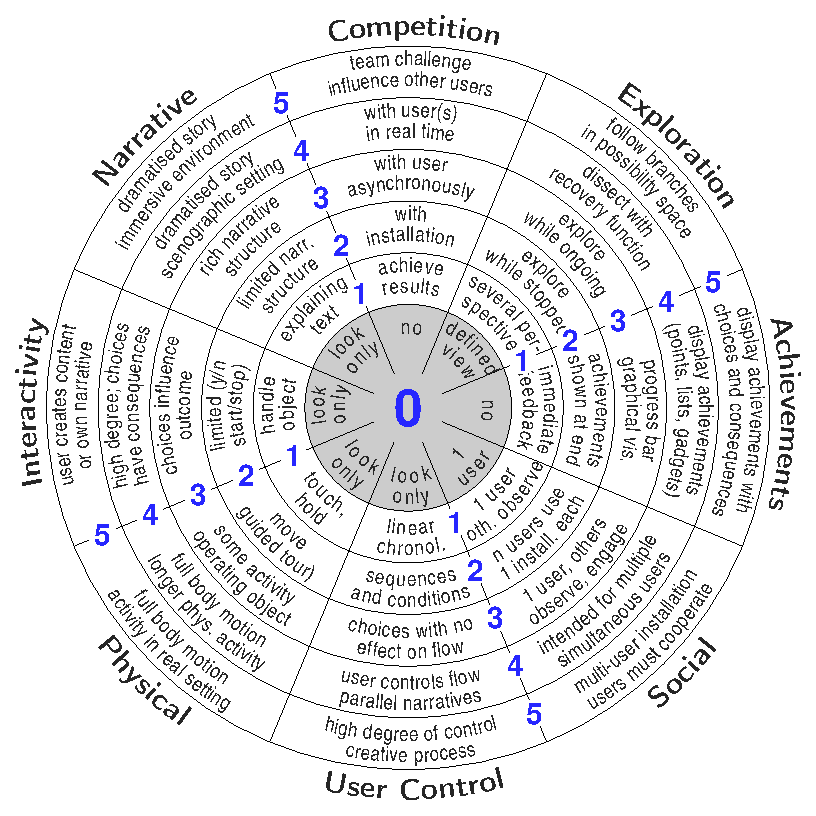
\includegraphics{figures/jVRARVestfold-ChartEPE}
\else
\begin{tikzpicture}[scale=1.75]
\path (\CNIPUSNL+\CNIPUSNLXX,\CNIPUSNL+\CNIPUSNLXX) --
(-\CNIPUSNL-\CNIPUSNLXX,\CNIPUSNL+\CNIPUSNLXX) --
(-\CNIPUSNL-\CNIPUSNLXX,-\CNIPUSNL-\CNIPUSNLXX) --
(\CNIPUSNL+\CNIPUSNLXX,-\CNIPUSNL-\CNIPUSNLXX);
% Draw background
\filldraw [fill=white!80!black] (0,0) circle (\CNIPUSNR/\CNIPUSNU*2);
\CNIPUSNdrawL
\filldraw [white!80!black,fill=white!80!black] (0,0) circle (\CNIPUSNR/\CNIPUSNU*0.7);
\renewcommand*{\mytextstyle}{\sffamily\large\bfseries\color{black!85}}
\renewcommand*{\myareatextstyle}{\fontfamily{phv}\fontseries{mc}\selectfont\footnotesize\color{black!85}}
\renewcommand*{\mynumbertextstyle}{\fontfamily{phv}\fontseries{mc}\selectfont\large\bfseries\color{blue!85}}
\renewcommand{\CNIPUSNlabeladjustment}{-2.0mm}
\renewcommand{\CNIPUSNraise}{-0.8ex}
%\fontfamily{phv}\fontseries{mc}\selectfont
\CNIPUSNtext{xxx}{1}{Competition}
\CNIPUSNtext{xxx}{2}{Narrative}
\CNIPUSNtext{xxx}{3}{Interactivity}
\CNIPUSNtext{xxx}{4}{Physical}
\CNIPUSNtext{xxx}{5}{User Control}
\CNIPUSNtext{xxx}{6}{Social}
\CNIPUSNtext{xxx}{7}{Achievements}
\CNIPUSNtext{xxx}{8}{Exploration}

% Competition
%\CNIPUSNareatext{xxx}{1}{{---}}{0}
\CNIPUSNareatext{xxx}{1}{no}{0.2}
%1
\CNIPUSNareatext{xxx}{1}{achieve}{1.4}
\CNIPUSNareatext{xxx}{1}{results}{1.0}
%2
\CNIPUSNareatext{xxx}{1}{with}{2.4}
\CNIPUSNareatext{xxx}{1}{installation}{2.0}
%3
\CNIPUSNareatext{xxx}{1}{with user}{3.4}
\CNIPUSNareatext{xxx}{1}{asynchronously}{3.0}
%4
\CNIPUSNareatext{xxx}{1}{with user(s)}{4.4}
\CNIPUSNareatext{xxx}{1}{in real time}{4.0}
%5
\CNIPUSNareatext{xxx}{1}{team challenge}{5.4}
\CNIPUSNareatext{xxx}{1}{influence other users}{5.0}

% Narrative
\CNIPUSNareatext{xxx}{2}{look}{0.4}
\CNIPUSNareatext{xxx}{2}{only}{-0.0}
%1
\CNIPUSNareatext{xxx}{2}{explaining}{1.4}
\CNIPUSNareatext{xxx}{2}{text}{1.0}
%2
\CNIPUSNareatext{xxx}{2}{limited narr.}{2.4}
\CNIPUSNareatext{xxx}{2}{structure}{2.0}
%3
\CNIPUSNareatext{xxx}{2}{rich narrative}{3.4}
\CNIPUSNareatext{xxx}{2}{structure}{3.0}
%4
\CNIPUSNareatext{xxx}{2}{dramatised story}{4.4}
\CNIPUSNareatext{xxx}{2}{scenographic setting}{4.0}
%5
\CNIPUSNareatext{xxx}{2}{immersive environment}{5.0}
\CNIPUSNareatext{xxx}{2}{dramatised story}{5.4}

% Interaction
\CNIPUSNareatext{xxx}{3}{look}{0.4}
\CNIPUSNareatext{xxx}{3}{only}{-0.0}
%1
\CNIPUSNareatext{xxx}{3}{handle}{1.4}
\CNIPUSNareatext{xxx}{3}{object}{1.0}
%2
\CNIPUSNareatext{xxx}{3}{limited (y/n}{2.4}
\CNIPUSNareatext{xxx}{3}{start/stop)}{2.0}
%3
\CNIPUSNareatext{xxx}{3}{choices influence}{3.4}
\CNIPUSNareatext{xxx}{3}{outcome}{3.0}
%4
\CNIPUSNareatext{xxx}{3}{high degree; choices}{4.4}
\CNIPUSNareatext{xxx}{3}{have consequences}{4.0}
%5
\CNIPUSNareatext{xxx}{3}{or own narrative}{5.0}
\CNIPUSNareatext{xxx}{3}{user creates content}{5.4}

% Physical
\CNIPUSNareatext{xxx}{4}{look}{0.0}
\CNIPUSNareatext{xxx}{4}{only}{0.4}
%1
\CNIPUSNareatext{xxx}{4}{touch,}{1.0}
\CNIPUSNareatext{xxx}{4}{hold}{1.4}
%2
\CNIPUSNareatext{xxx}{4}{move}{2.0}
\CNIPUSNareatext{xxx}{4}{guided tour)}{2.4}
%3
\CNIPUSNareatext{xxx}{4}{some activity}{3.0}
\CNIPUSNareatext{xxx}{4}{operating object}{3.4}
%4
\CNIPUSNareatext{xxx}{4}{full body motion}{4.0}
\CNIPUSNareatext{xxx}{4}{longer phys. activity}{4.4}
%5
\CNIPUSNareatext{xxx}{4}{full body motion}{5.0}
\CNIPUSNareatext{xxx}{4}{activity in real setting}{5.4}

% User Control
\CNIPUSNareatext{xxx}{5}{look}{0.0}
\CNIPUSNareatext{xxx}{5}{only}{0.4}
%1
\CNIPUSNareatext{xxx}{5}{linear}{1.0}
\CNIPUSNareatext{xxx}{5}{chronol.}{1.4}
%2
\CNIPUSNareatext{xxx}{5}{sequences}{2.0}
\CNIPUSNareatext{xxx}{5}{and conditions}{2.4}
%3
\CNIPUSNareatext{xxx}{5}{choices with no}{3.0}
\CNIPUSNareatext{xxx}{5}{effect on flow}{3.4}
%4
\CNIPUSNareatext{xxx}{5}{user controls flow}{4.0}
\CNIPUSNareatext{xxx}{5}{parallel narratives}{4.4}
%5
\CNIPUSNareatext{xxx}{5}{high degree of control}{5.0}
\CNIPUSNareatext{xxx}{5}{creative process}{5.4}


% Social
\CNIPUSNareatext{xxx}{6}{1}{0.0}
\CNIPUSNareatext{xxx}{6}{user}{0.4}
%1
\CNIPUSNareatext{xxx}{6}{1 user}{1.0}
\CNIPUSNareatext{xxx}{6}{oth.~observe}{1.4}
%2
\CNIPUSNareatext{xxx}{6}{n users use}{2.0}
\CNIPUSNareatext{xxx}{6}{1 install.~each}{2.4}
%3
\CNIPUSNareatext{xxx}{6}{1 user, others}{3.0}
\CNIPUSNareatext{xxx}{6}{observe, engage}{3.4}
%4
\CNIPUSNareatext{xxx}{6}{intended for multiple}{4.0}
\CNIPUSNareatext{xxx}{6}{simultaneous users}{4.4}
%5
\CNIPUSNareatext{xxx}{6}{multi-user installation}{5.0}
\CNIPUSNareatext{xxx}{6}{users must cooperate}{5.4}

% Achievements
%\CNIPUSNareatext{xxx}{7}{{---}}{0}
\CNIPUSNareatext{xxx}{7}{no}{0.2}
%\CNIPUSNareatext{xxx}{7}{look}{0.4}
%\CNIPUSNareatext{xxx}{7}{only}{-0.1}
%1
\CNIPUSNareatext{xxx}{7}{immediate}{1.4}
\CNIPUSNareatext{xxx}{7}{feedback}{1.0}
%2
\CNIPUSNareatext{xxx}{7}{achievements}{2.4}
\CNIPUSNareatext{xxx}{7}{shown at end}{2.0}
%3
\CNIPUSNareatext{xxx}{7}{progress bar}{3.4}
\CNIPUSNareatext{xxx}{7}{graphical vis.}{3.0}
%4
\CNIPUSNareatext{xxx}{7}{display achievements}{4.4}
\CNIPUSNareatext{xxx}{7}{(points, lists, gadgets)}{4.0}
%5
\CNIPUSNareatext{xxx}{7}{display achievements with}{5.4}
\CNIPUSNareatext{xxx}{7}{choices and consequences}{5.0}

% Explore
%\CNIPUSNareatext{xxx}{8}{{---}}{0}
\CNIPUSNareatext{xxx}{8}{defined}{0.4}
\CNIPUSNareatext{xxx}{8}{view}{0.0}
%1
\CNIPUSNareatext{xxx}{8}{several per-}{1.4}
\CNIPUSNareatext{xxx}{8}{spectives}{1.0}
%2
\CNIPUSNareatext{xxx}{8}{explore}{2.4}
\CNIPUSNareatext{xxx}{8}{while stopped}{2.0}
%3
\CNIPUSNareatext{xxx}{8}{explore}{3.4}
\CNIPUSNareatext{xxx}{8}{while ongoing}{3.0}
%4
\CNIPUSNareatext{xxx}{8}{dissect with}{4.4}
\CNIPUSNareatext{xxx}{8}{recovery function}{4.0}
%5
\CNIPUSNareatext{xxx}{8}{follow branches}{5.4}
\CNIPUSNareatext{xxx}{8}{in possibility space}{5.0}


\CNIPUSNNumbersL{3}
\CNIPUSNNumbersL{7}
\CNIPUSNNumbersL{1}
\CNIPUSNNumbersL{5}
%\filldraw [fill=white!80!black] (0,0) circle (\CNIPUSNR/\CNIPUSNU*1);
%\draw (0,0) node {0--5};
\node at (0,0)
%      [circle,inner sep=0pt, minimum size=0.4em,draw=white,fill=white]
      {\mynumbertextstyle\huge 0};
\end{tikzpicture}
\fi
%\end{center}
\caption{The dimensions of the \EP explained with short
  definitions. To define the value of a property, find the adjacent
  number of the phrases that fit best.}\label{fig:engagementprofile}
\end{figure}
